\chapter{Developing The Codebase}\label{ch:developingthecodebase}
This chapter will discuss the development practices encountered during the project and a walkthrough of setting up an environment.
Details on the set up and reasoning behind using specific development environments will be given along with a look at the open source contributions made.
A brief look at version control will also show how code is developed to be sustainable and reproducible.

\section{Codebase Contributions}
Throughout the project I had split time between writing my own code and expanding the Axelrod Dojo codebase. 
In modern software development there is a commitment in the developer community to track and reuse as much code as possible, typically using a version control system such as Git or Subversion.
The majority of open source community development is conducted on GitHub\cite{GitHub} using Git, the Axelrod libraries, along with most other libraries I used, are hosted here.

When writing code in a professional environment there is a predetermined scope that all parties agree upon before the work commences.  This, however, is not the case for research development which is more organic;
final products that are created when conducting research for papers are highly personalised and typically cannot be used in other areas.
This leads to more flexible products that operate more as platforms or tools for further research, this is why the Axelrod, Axelrod Dojo and other libraries mentioned in table~\ref{table:functionalLibrares} exist.
My final code will only be used for researching the IPD in my projects specific direction, this meant extending the platforms to handle what I needed them to do, subsection~\ref{ssec:versioncontrol} looks into how this was completed in my project.

\subsection{Version Control}\label{ssec:versioncontrol}
During the project I created a `fork' of the Axelrod Dojo in order to add content to the open source community. 
This resulted in using Git to create a new `branch' on which to write my code before asking the owners of the repository to pull my work back into the core product using a `pull request'(PR).
The PR opened for my code\footnote{https://github.com/Axelrod-Python/axelrod-dojo/pull/45} resulted in changes to 457 lines of code and 14 files, adding classes and fixing bug that had been previously flagged.
Figure~\ref{fig:PR-open} shows the initial scope of the PR and Figure~\ref{fig:commit-log} shows a section of the commits made before merging the branch.

\begin{figure}[ht]
    \centering
    \begin{minipage}{0.48\textwidth}
        \centering
        \includegraphics[width=1.0\textwidth, center]{./img/vcs/PR-Open.png}
        \caption{Description and commits for PR on Github}\label{fig:PR-open}
    \end{minipage}\hfill
    \begin{minipage}{0.48\textwidth}
        \centering
        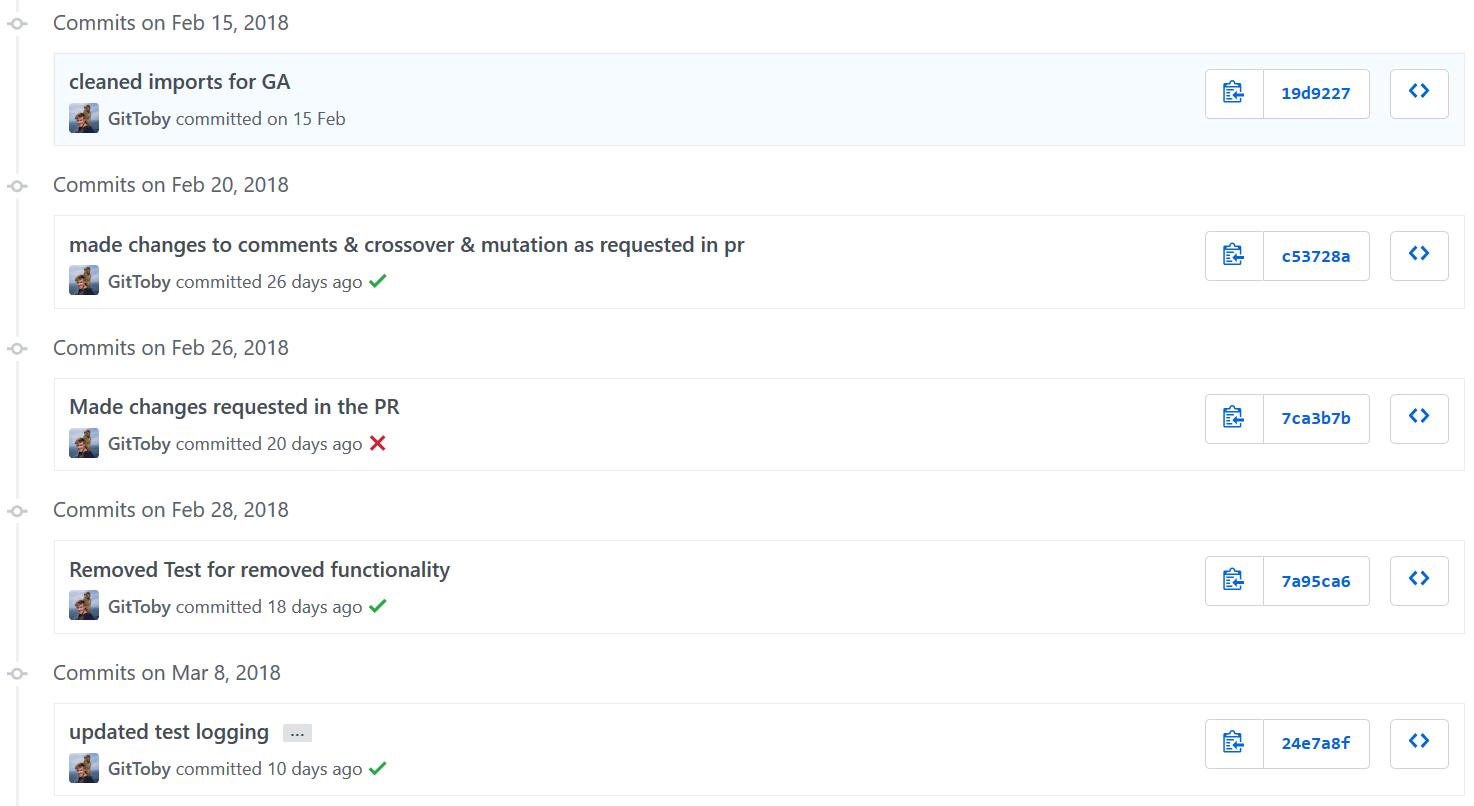
\includegraphics[width=1.0\textwidth, center,keepaspectratio]{./img/vcs/commit-log.png}    
        \caption{Tail of code commit log as shown on Github}\label{fig:commit-log}
    \end{minipage}
\end{figure}

After a request is opened there is a period of reviews by the owners, this is to ensure code quality and scope coverage. 
As my work progressed I continued to add to the PR which lead to more and more requests being added for features that fell outside the scope of the PR.
Eventually we decided to create another fork of the PR that contained specialist code for my project that would not benefit the codebase as a whole.
Figures~\ref{fig:PR-discussion} \&~\ref{fig:PR-scope-discussion} show examples of requests and discussions around features and code quality.
Because of this review process the overall quality of the codebase can be kept high and the owners can decide on how their platforms are developed.

\begin{figure}[ht]
    \centering
    \begin{minipage}{0.48\textwidth}
        \centering
        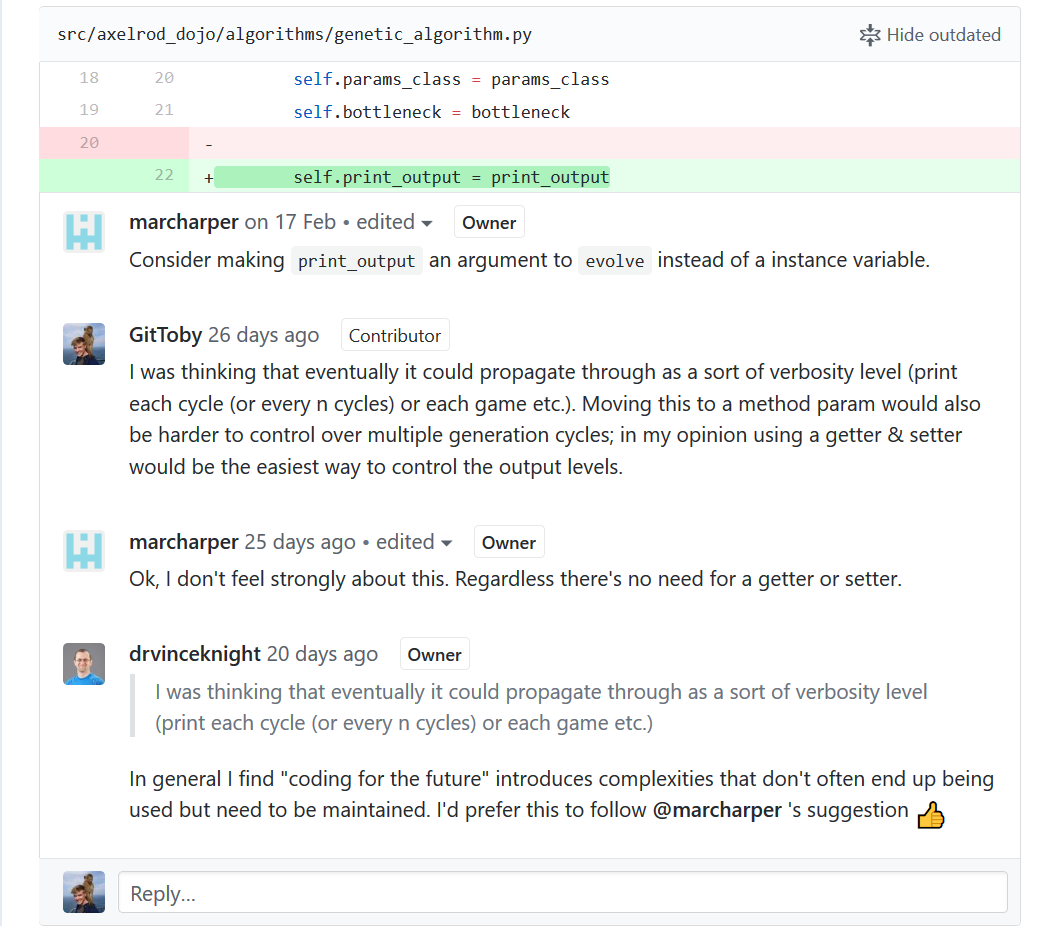
\includegraphics[width=1.0\textwidth, center,keepaspectratio]{./img/vcs/feature-discussion.png}
        \caption{Feature discussions in PR on GitHub}\label{fig:PR-discussion}
    \end{minipage}\hfill
    \begin{minipage}{0.48\textwidth}
        \centering
        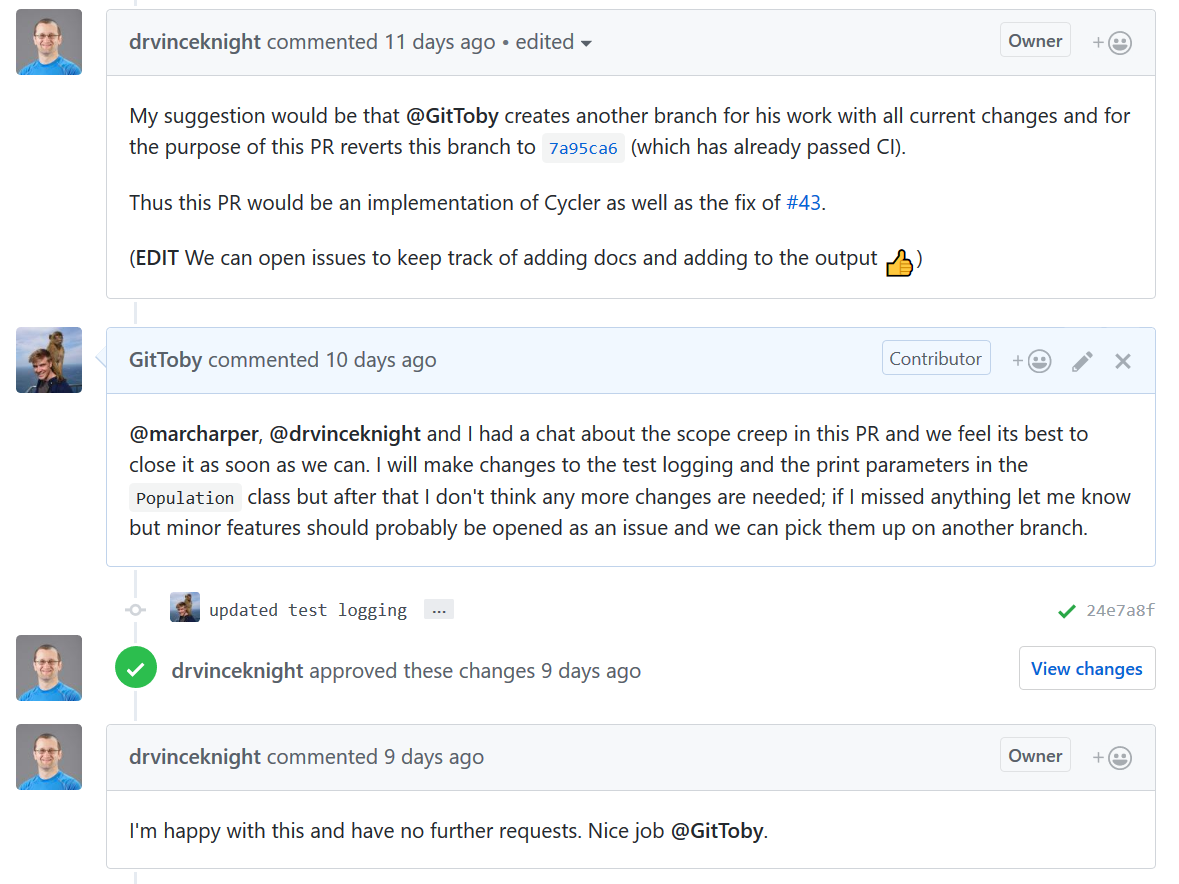
\includegraphics[width=1.0\textwidth, center,keepaspectratio]{./img/vcs/scope-discussion.png}    
    \caption{Scope Discussion in PR on GitHub}\label{fig:PR-scope-discussion}
    \end{minipage}
\end{figure}

\subsection{Testing}\label{ssec:testing}
Code testing and version control go hand in hand. 
When new releases of code are made it is important to ensure that the new changes dont break previous functionality.
This is kept in check by the presence of continues integrations (CI) and test environments.
As of this project the CI for the Axelrod Dojo keeps the libraries tests running on a linux environment and the output fed to the Github page.
During my development I had to implement tests for any functionality I wrote to ensure the library still worked as intended.
Following the mixed practice of test driven design (TDD) and behaviour driven design (BDD) the code written to extend the Axelrod Dojo had tests to cover examples of what happens in a production environment~\cite{hong2015top, prlic2012ten, sandve2013ten}.
Snippet~\ref{code:test-example} shows an example of a test.

\begin{figure}[ht]
    \inputminted{python}{code_snippets/dev-examples/example-test.py}
    \caption{An Example of a test in the Axelrod Dojo}\label{code:test-example}
\end{figure}

\section{Libraries And External Modules}
\paragraph{Main Research Libraries}
\begin{itemize}
    \item \textbf{Axelrod} --- Used for the core of the prisoners dilemma and iterated prisoners dilemma functionality code.\cite{axelrodproject}
    \item \textbf{Axelrod Dojo} --- Applied machine learning techniques that revolve around generating solutions to questions relating to the Axelrod library~\cite{dojoV008}.
\end{itemize}

\paragraph{Functional libraries}
Table~\ref{table:functionalLibrares} shows the external functional libraries used, while Table~\ref{table:builtinmodules} shows the internal python built in modules that where leveraged during development.
These are libraries which are not involved in the core functionality of the IPD\@.
\begin{table*}[ht]
    \centering
    \begin{tabular}{ccc}
        \toprule
        Library & Reason & Reference\\
        \midrule
        \textbf{matplotlib pyplot} & For plotting graphs and images with data & \cite{hunter2007matplotlib}\\
        \textbf{pandas} & For data manipulation. & \cite{PandasGithub,Mckinney2010pandas}\\
        \textbf{numpy} & For reducing complexity of numerical calculations.& \cite{oliphant2006numpy}\\
        \textbf{SciKit Learn} & For existing ML tools. & \cite{pedregosa2011scikit}\\
        \bottomrule
    \end{tabular}
    \caption{Functional Python libraries for analysis}\label{table:functionalLibrares}
\end{table*}
\begin{table*}[ht]
    \centering
    \begin{tabular}{cc}
        \toprule
        Module & Reason\\
        \midrule
        \textbf{os} & For operating system functionality.\\
        \textbf{time} & For time calculations.\\
        \textbf{itertools} & For easier iterations over data structures.\\
        \bottomrule
    \end{tabular}
    \caption{Internal built in python modules used}\label{table:builtinmodules}
\end{table*}

\section{Reproducing Analysis}\label{subsec:settingUpAResearchEnvironment}
A mix of Jupyter Notebooks and integrated development environments\footnote{Pycharm Professional Edition and Microsoft VS Code.} were used to write and execute code.
The main analysis was run using a factory class pattern, called \mintinline{python}{AnalysisRun} in the \mintinline{python}{full_analysis} module, show in Figure~\ref{apcode:AnalysisRun.py}.
This class was used to wrap a query to the Axelrod Dojo functionality and subsequently to the Axelrod Library in such a way that was easy to control batch executions.

The analysis itself was done using native multi-threading on a Linux OS to improve individual opponent analysis run times and the overall scalability of the project.
.This tutorial will also assume you're working with a local development station;
analysis on remote cloud instances of Jupyter Notebooks is possible but the set up is different.

\paragraph{Installing Basic Libraries}
Your first step should be to download and install the Anaconda distribution for your OS here: https://www.anaconda.com/download/.
This will allow you to use the integrated c++ libraries python has to offer without needing to mess about too much.
Anaconda also has them majority of Functional Libraries above and Jupyter Notebooks pre installed to make setting up much easier.
From here, follow the instructions the install wizard has to add any environment variables to allow CMD/Bash access to binaries.

Installing the Axelrod and Axelrod Dojo libraries uses the pip tool that already comes with Anaconda and should be ready to execute after the last step.Running `pip install axelrod' then `pip install axelrod-dojo' will install these.

Once this is installed the \mintinline{python}{full\_analysis.py} file has to be downloaded from GitHub\footnote{https://github.com/GitToby/FinalYearProject}, it can be found in the code directory.This can just be copied and pasted if needed all were interested in is the class to generate a sequence for an opponent.

\paragraph{Running a Test}
Figure~\ref{code:analysisExample} is some sample code that will run an analysis with the following settings:
\begin{itemize}
    \item Override the default mutation frequency of \(0.1\) to \(0.3\).
    \item Set the prefix for all the files to be `example-'.
    \item Analysing 3 opponents.(Random will have multiple instances for different seeds.) 
\end{itemize}
\begin{figure}[ht]
    \centering
    \inputminted{python}{code_snippets/analysisExample.py}
    \caption{Code to create a sequence result to optimise best score for 3 opponents}\label{code:analysisExample}
\end{figure}

After it has run the generated data output should be stored in the `./output' directory.
If the code fails to run there may be issues with this directory being created.
There should be multiple output files, each with one opponents evolution stages through the generations.

\paragraph{Cloud Notebook Setup} 
If you want to use a Cloud service, such as Azure Notebooks or AWS Sagemaker, the set up is similar to the above just executed differently.
Installing Anaconda is not needed, the environment has the required installs.
Using pip to install the Axelrod libraries and download the full analysis script can be done in an integrated web terminal or directly in a notebook.
Figure~\ref{code:jupyterExample} shows and example in azure, copy these in your top few cells of your jupyter notebook and it will work as required.

\begin{figure}[ht]
    \inputminted{python}{code_snippets/dev-examples/jupyterCells.py}
    \caption{Cells for creating the jupyter instance of a research environment}\label{code:jupyterExample}
\end{figure}

\section{Conclusion}
In this Chapter we covered the contributions needed to the Axelrod Dojo to carry on the work described in this report. Moreover, we covered the procedure of implementing and contributing to an open source package.
Of the learning that was complexity during the project, learning a new version control system was the hardest along with handling the organic growth of the project.
While writing code there where sections that needed changing or removing, however there was no scope or predetermined set of outcomes causing my own analysis notebooks to swell and become unwieldy at times.
These problems were solved by selectively isolating work and levering 3rd party libraries more.

The final codebase contributions were a success and version 0.0.8 of the Axelrod Dojo has been released to the python installer package, `pip'~\cite{dojoV008}.
Following the steps in Section~\ref{subsec:settingUpAResearchEnvironment} will allow a working environment to be set up on any platform, letting this experiment be repeated.
Providing a reproducible experiment allows the open source and research communities independently verify any findings in this work to ensure a robust foundation for future work.
All finalised notebooks and final code are published online on GitHub, urls can be found in Appendix~\ref{apndx:resources}.